% \documentclass{WHUBachelor}% 选项 forprint: 交付打印时添加, 避免彩色链接字迹打印偏淡. 即使用下一行:
\documentclass[forprint]{myreport}
\usepackage{subfig}
\usepackage{listings}
\lstdefinestyle{lfonts}{
  basicstyle = \footnotesize\ttfamily,
  stringstyle = \color{purple},
  keywordstyle = \color{blue!60!black}\bfseries,
  commentstyle = \color{olive}\scshape,
}
\lstdefinestyle{lnumbers}{
  numbers = left,
  numberstyle = \tiny,
  numbersep = 1em,
  firstnumber = 1,
  stepnumber = 1,
}
\lstdefinestyle{llayout}{
  breaklines = true,
  tabsize = 2,
  columns = flexible,
}
\lstdefinestyle{lgeometry}{
  xleftmargin = 20pt,
  xrightmargin = 0pt,
  frame = tb,
  framesep = \fboxsep,
  framexleftmargin = 20pt,
}
\lstdefinestyle{lgeneral}{
  style = lfonts,
  style = lnumbers,
  style = llayout,
  style = lgeometry,
}
\lstdefinestyle{c}{
	language = {c},
	style = lgeneral,
}


\begin{document}
%%%%%%%%%%%%%%%%%%%%%%%%%%%%%%%%%%%%%%%%%%%%%%%%%%%%%%%%%%%%%%%%%%%%%%%%%%%%
% 封面
%%%%%%%%%%%%%%%%%%%%%%%%%%%%%%%%%%%%%%%%%%%%%%%%%%%%%%%%%%%%%%%%%%%%%%%%%%%%
\title{计算机图形学 HW2}
\Cschoolname{数据科学与计算机学院}          % 学院名
\Cmajor{计算机科学与技术}                  % 专业中文名
\StudentNumber{16337237} % 填写自己的学号
\author{王永锋}                            % 作者名字
\Csupervisor{苏卓}        %指导教师中文名、职称
\date{二〇一八年四月三十日}                % 日期, 要注意和英文日期一致!!
\pdfbookmark[0]{封面}{title}         % 封面页加到 pdf 书签
\maketitle
\frontmatter
%%%%%%%%%%%%%%%%%%%%%%%%%%%%%%%%%%%%%%%%%%%%%%%%%%%%%%%%%%%%%%%%%%%%%%%%%%%%
% 目录
%%%%%%%%%%%%%%%%%%%%%%%%%%%%%%%%%%%%%%%%%%%%%%%%%%%%%%%%%%%%%%%%%%%%%%%%%%%%
% 把目录加入到书签
\pagenumbering{Roman}              % 正文之前的页码用大写罗马字母编号.
\pdfbookmark[0]{目录}{toc}
\tableofcontents
%% 以下是正文
\mainmatter 
%%%%%%%%%%%%%%%%%%%%%%%%%%%%%%%%%%%%%%%%%%%%%%%%%%%%%%%%%%%%%%%%%%%%%%%%%%%%
% 正文
%%%%%%%%%%%%%%%%%%%%%%%%%%%%%%%%%%%%%%%%%%%%%%%%%%%%%%%%%%%%%%%%%%%%%%%%%%%%

\chapter{配置开发环境}

\section{开发环境}

本作业在Window10下使用基于MinGW的gcc编译器编译运行。

\section{依赖第三方库}

参考自教程\cite{r1}的环境,在第三方的OpenGL窗口管理程序库中,我选择了glfw并配置在我的项目文件夹中。除此之外,为了得到OpenGL程序中函数的具体位置,我还使用了GLAD来进行函数的定位。在实现图2的过程中,我还用到了glm用于计算旋转、平移、投影矩阵。

%\usepackage{changepage}
%\usepackage{rotating}
%\begin{sidewaystable}[htp]
\begin{figure}[htp]
  %\begin{adjustwidth}{-1.5cm}{-1cm}
  \centering
  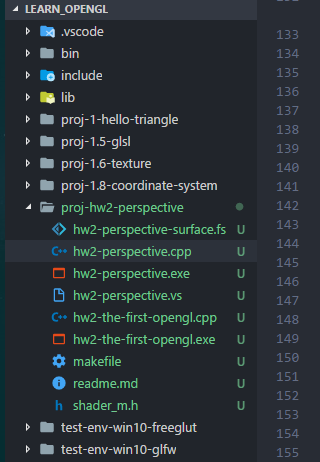
\includegraphics[width=6cm]{"figure/2018-05-01-16-04-36.png"}
  \caption{开发环境图示}
  \label{fig:env}
  %\end{adjustwidth}
\end{figure}





\chapter{图1效果实现}

\section{相关文件说明}

实现效果的源代码文件为“hw2-the-first-opengl.cpp",可执行文件为"hw2-the-first-opengl.exe"。由于通过静态链接库的方式进行编译,因此可直接运行。

\section{部分设计细节}

在实现这一个矩形的过程中,我参考了一部分来自教程\cite{r1}的代码。

代码主要分为这几个部分:

\begin{itemize}
  \item 使用glfw创建窗口
  \item 使用glad导入opengl函数
  \item 编译着色器(着色器的编写)
  \item 绑定顶点缓冲对象,顶点数组对象
  \item 渲染循环
\end{itemize}

\subsection{细节1}

需要注意的一个细节是,OpenGL中的绘制对象只有三种:点,线,三角形。那要如何绘制矩形呢?教程\cite{r1}中给出了一个解决方法:使用两个三角形来拼出一个矩形。\footnote{事实上,后来上网一搜,发现无论是多复杂的图形,都需要使用三角形来拼出来}。

因此在初始化顶点数组的时候,便初始化了两个三角形。



%\usepackage{listings}
\begin{lstlisting}[style = c]
    float vertices_white[] = {
      // 第一个三角形
      0.5f, 0.5f, 0.0f,   // 右上角
      0.5f, -0.5f, 0.0f,  // 右下角
      -0.5f, 0.5f, 0.0f,  // 左上角
      // 第二个三角形
      0.5f, -0.5f, 0.0f,  // 右下角
      -0.5f, -0.5f, 0.0f, // 左下角
      -0.5f, 0.5f, 0.0f   // 左上角
    };
\end{lstlisting}



\section{运行截图}

运行\textbf{hw2-the-first-opengl.exe},结果如\autoref{fig:screenshot1}所示。

%\usepackage{changepage}
%\usepackage{rotating}
%\begin{sidewaystable}[htp]
\begin{figure}[htp]
  %\begin{adjustwidth}{-1.5cm}{-1cm}
  \centering
  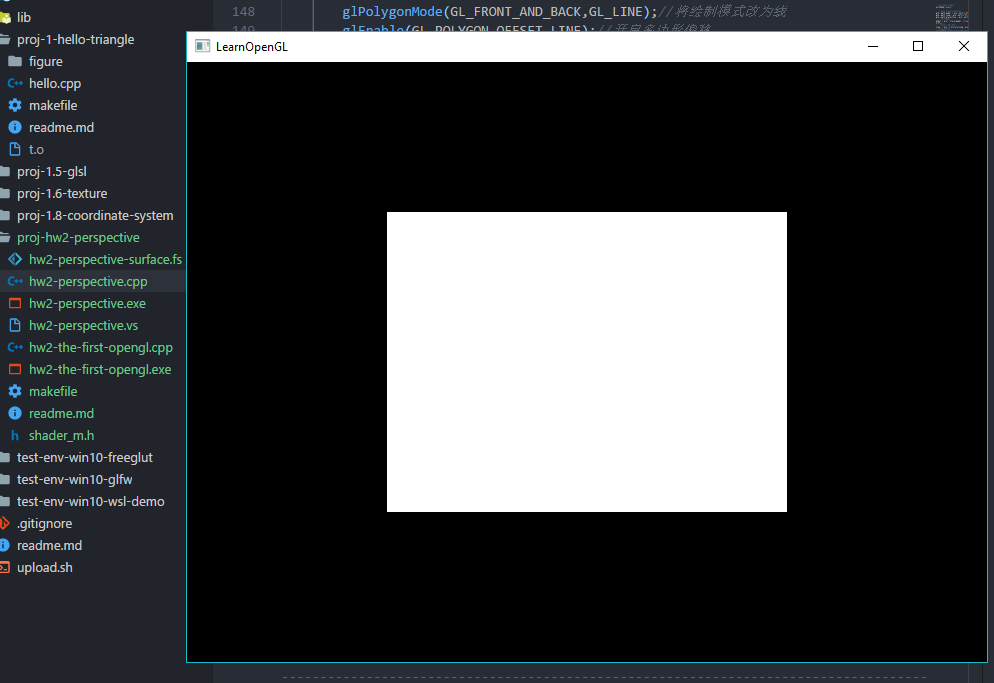
\includegraphics[width=13cm]{"./figure/2018-05-01-15-06-43.png"}
  \caption{运行截图1}
  \label{fig:screenshot1}
  %\end{adjustwidth}
\end{figure}

\chapter{图2效果实现}

\section{相关文件说明}

实现图2过程中,使用了以下文件。
其中可执行文件\textbf{hw2-perspective.exe}直接打开运行即可。

%\usepackage{listings}
\begin{lstlisting}[style = c]
  └── shader_m.h                // 用于读取着色器
  ├── hw2-perspective.cpp       // 主要源代码
  ├── hw2-perspective.vs        // 顶点着色器
  ├── hw2-perspective-surface.fs// 片段着色器
  ├── makefile                  // 用于编译程序
  ├── hw2-perspective.exe       // 可执行文件
\end{lstlisting}

\section{部分设计细节}

在实现图2的过程中,我主要遇到了一下问题:

\begin{itemize}
  \item 坐标转换的实现
  \item 在显示正方体的同时显示边缘
\end{itemize}

\subsection{坐标转换}

要将一个正方体显示在屏幕上,一个关键的步骤就是将这个物体的各个顶点转变为在屏幕上的一个个像素,这其中,就需要用到坐标变换。

在我的程序中,坐标变换的实现。

%\usepackage{listings}
\begin{lstlisting}[style = c]
  glm::mat4 model = glm::mat4(1.0f);
  glm::mat4 view = glm::mat4(1.0f);
  glm::mat4 projection = glm::mat4(1.0f);
  // 旋转矩阵,实现随时间旋转
  model = glm::rotate(model, (float)glfwGetTime(), glm::vec3(-0.5f, 0.5f, 0.0f));
  // 将物体向前平移三个单位,方便观察
  view  = glm::translate(view, glm::vec3(0.0f, 0.0f, -3.0f));
  // 设置投影,角度为45度
  projection = glm::perspective(glm::radians(45.0f), (float)SCR_WIDTH / (float)SCR_HEIGHT, 0.1f, 100.0f);
\end{lstlisting}

这些变换矩阵,最终在顶点着色器中起作用,如以下代码第14行所示。

%\usepackage{listings}
\begin{lstlisting}[style = c]
  #version 330 core
  layout (location = 0) in vec3 aPos;
  
  out vec4 outColor;
  
  uniform mat4 model;
  uniform mat4 view;
  uniform mat4 projection;
  uniform vec4 myColor;
  
  void main()
  {
    # 计算得到顶点变换后的坐标
    gl_Position = projection * view * model * vec4(aPos, 1.0f);
    outColor = myColor;	
  }
\end{lstlisting}

\subsection{正方体与轮廓线同时显示}

看到老师的实例图中,正方体不仅着了色,还有清晰的轮廓线。在我的实现中,我并不清楚如何将轮廓线画出来,于是便开始各种尝试。

我曾经试过通过修改着色器,让着色器对边缘着上其他颜色,结果却变成了一个具有渐变颜色的正方体,这应该是由于着色器本身就具有片段插值的功能,我暂时还不会干预着色器的这种行为,于是便寻找其他方法。

在博客\cite{r2}中,热心网友提出了一种方法,通过修改全局配置的方法,将绘制面改为绘制轮廓线。这样子只需要在绘制完所有图像后,修改状态位绘制轮廓线,再绘制一次图像即可。参考他的视线,我在渲染循环中增加了绘制轮廓线的过程。效果其实并不好,在正方体旋转的过程中,会出现一闪一闪的情况,而且还一定会画出正方形中间的斜线(那些我不想画出来的轮廓线)。效果如\autoref{fig:screen2}所示。


其实还有一种办法,就是再创建多几个对象,然后使用绘制直线的命令将轮廓线画出来,再启动深度检测,可能也行,不过这种由于实现比较繁琐,就没有继续实现下去。

\section{运行截图}

%\usepackage{subfig}
\begin{figure}[htbp]
\centering
\subfloat[运行截图2-1]{
  \label{fig:screen2}
  \begin{minipage}[t]{0.5\linewidth}
    \centering
    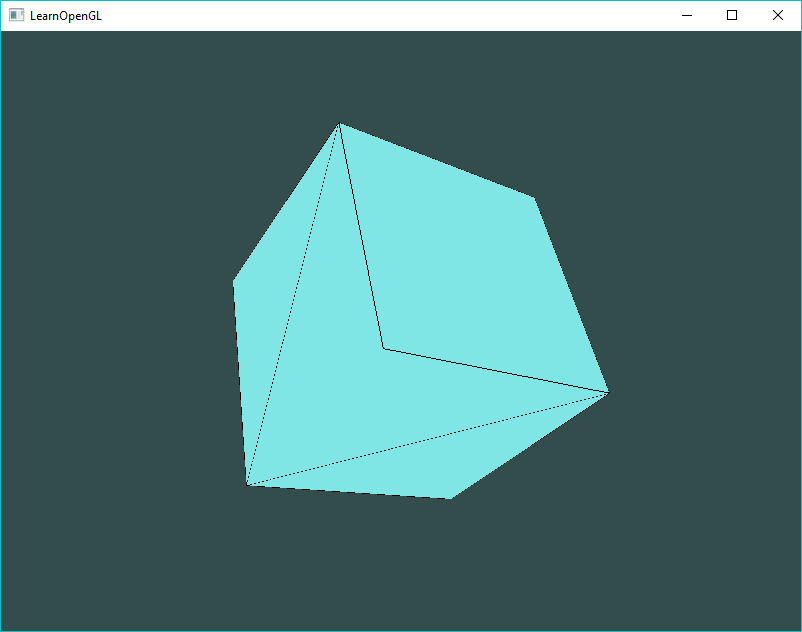
\includegraphics[width=0.9\textwidth]{figure/2018-05-01-15-27-57.png}
  \end{minipage}
}
\subfloat[运行截图2-2]{%the name of subfloat
  \label{fig:screen3}
  \begin{minipage}[t]{0.5\linewidth}
    \centering
    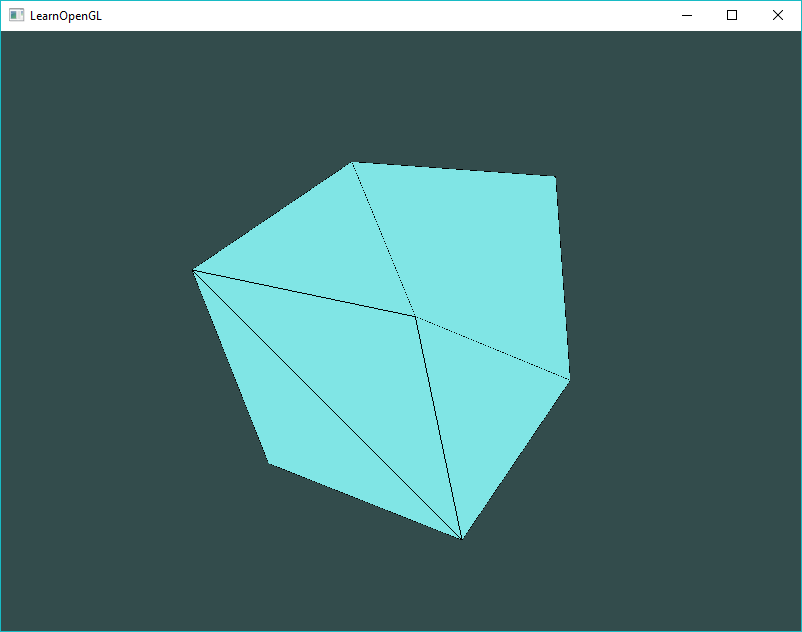
\includegraphics[width=0.9\textwidth]{figure/2018-05-01-15-28-40.png}
  \end{minipage}
}
\caption{运行截图2}
\end{figure}

\chapter{作业感想}

以前由于python课程项目要做3D建模的缘故,接触过一些关于OpenGL的知识,不过那时候看的是关于固定渲染管线的实现,对于目前的现代OpenGL方法而言并不熟悉。

这一次看的OpenGL教程,一上来就讲固定渲染管线隐藏了太多细节,让我学现代OpenGL,使用OpenGL的核心模式编程,难度曲线陡升。毕竟,连渲染一条简单的直线,我都必须要自己编写着色器,去给我的顶点着色,更别提渲染更复杂的带有纹理的立体图形了。

这一个作业中的代码,其实有挺多都有参考教程的实例代码(到现在想想,我自己可能还不能够不看示例代码就能够完整的写出这些程序),可以说这个教程对我的学习起到了莫大的帮助,现在我至少是能够看懂教程提供的示例代码,并且通过修改示例代码的方式实现自己想要的功能。

不过,这一次作业花的时间太长了,从开始看教程到完成作业,花了将近一天时间,才把OpenGL的核心模式看懂一部分,理解了OpenGL的运行逻辑。为了保证开发效率,不知道要不要转投python的怀抱诶。

%%%%%%%%%%%%%%%%%%%%%%%%%%%%%%%%%%%%%%%%%%%%%%%%%%%%%%%%%%%%%%%%%%%%%%%%%%%%
% 参考文献
%%%%%%%%%%%%%%%%%%%%%%%%%%%%%%%%%%%%%%%%%%%%%%%%%%%%%%%%%%%%%%%%%%%%%%%%%%%%
% \cleardoublepage\phantomsection
% \addcontentsline{toc}{chapter}{参考文献}

% \bibliography{opsystem}
% \bibliographystyle{unsrt}

\begin{thebibliography}{00}
  \bibitem{r1} OpenGL教程:https://learnopengl-cn.github.io/
  \bibitem{r2} CSDN博客:OpenGL:三维模型,模型网格点与面片同时显示,模型网格轮廓线与面片同时显示。\url{https://blog.csdn.net/hw140701/article/details/78913660}
  %   \bibitem{r3} 邓建松等, 《\LaTeXe~科技排版指南》, 科学出版社.
%   \bibitem{r4} 吴凌云, 《CTeX~FAQ (常见问题集)》, \textit{Version~0.4}, June 21, 2004.
%   \bibitem{r5} Herbert Vo\ss, Mathmode, \url{http://www.tex.ac.uk/ctan/info/math/voss/mathmode/Mathmode.pdf}.
\end{thebibliography}
%%%%%%%%%%%%%%%%%%%%%%%%%%%%%%%%%%%%%%%%%%%%%%%%%%%%%%%%%%%%%%%%%%%%%%%%%%%%
% 附录
%%%%%%%%%%%%%%%%%%%%%%%%%%%%%%%%%%%%%%%%%%%%%%%%%%%%%%%%%%%%%%%%%%%%%%%%%%%%
% \appendix

% \chapter{文件的组织}

\cleardoublepage
\end{document}